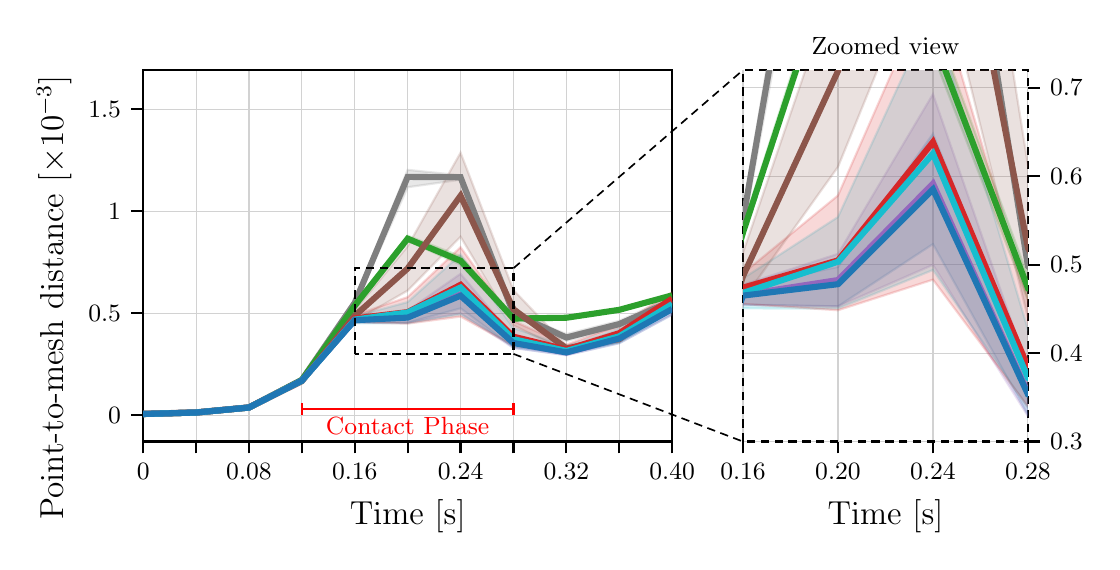
\begin{tikzpicture}

\definecolor{crimson2143940}{RGB}{214,39,40}
\definecolor{forestgreen4416044}{RGB}{44,160,44}
\definecolor{darkturquoise23190207}{RGB}{23,190,207}
\definecolor{gray127}{RGB}{127,127,127}
\definecolor{lightgray204}{RGB}{204,204,204}
\definecolor{mediumpurple148103189}{RGB}{148,103,189}
\definecolor{sienna1408675}{RGB}{140,86,75}
\definecolor{steelblue31119180}{RGB}{31,119,180}

% Plot content, shared by the full view and the zoomed view
\newcommand{\ablationcontent}{%
% Shaded areas
% No Context
\path [draw=gray127, fill=gray127, opacity=0.18]
(axis cs:0,8.07295291394894e-06)
--(axis cs:0,5.12359331139578e-06)
--(axis cs:1,1.24465407043317e-05)
--(axis cs:2,3.70405652006411e-05)
--(axis cs:3,0.000170184562616669)
--(axis cs:4,0.000538726298991605)
--(axis cs:5,0.00111711371160709)
--(axis cs:6,0.0011539952494968)
--(axis cs:7,0.000493944165682478)
--(axis cs:8,0.000363235438599077)
--(axis cs:9,0.000430213335330336)
--(axis cs:10,0.000541865832110489)
--(axis cs:10,0.000579285589992651)
--(axis cs:10,0.000579285589992651)
--(axis cs:9,0.000462110629396193)
--(axis cs:8,0.000397154613974635)
--(axis cs:7,0.000502686903510039)
--(axis cs:6,0.00117566139379051)
--(axis cs:5,0.00120230794382223)
--(axis cs:4,0.000562686173348084)
--(axis cs:3,0.000175566404236633)
--(axis cs:2,3.94724731199858e-05)
--(axis cs:1,1.48931526597096e-05)
--(axis cs:0,8.07295291394894e-06)
--cycle;
% Oracle
\path [draw=forestgreen4416044, fill=forestgreen4416044, opacity=0.18]
(axis cs:0,5.02822931252922e-06)
--(axis cs:0,5.00629528346508e-06)
--(axis cs:1,1.22442673364276e-05)
--(axis cs:2,3.64980695599115e-05)
--(axis cs:3,0.000170152035236697)
--(axis cs:4,0.000531509038712556)
--(axis cs:5,0.000854251318701245)
--(axis cs:6,0.000737646454490459)
--(axis cs:7,0.00045989315263796)
--(axis cs:8,0.000471600066430256)
--(axis cs:9,0.000512676674770773)
--(axis cs:10,0.000583336630952544)
--(axis cs:10,0.00059101728056703)
--(axis cs:10,0.00059101728056703)
--(axis cs:9,0.000520028840073792)
--(axis cs:8,0.000481395700517169)
--(axis cs:7,0.00048684069643059)
--(axis cs:6,0.000778906577484122)
--(axis cs:5,0.000879407519557844)
--(axis cs:4,0.000544052049326638)
--(axis cs:3,0.000173569310650237)
--(axis cs:2,3.67153696726064e-05)
--(axis cs:1,1.23036071607885e-05)
--(axis cs:0,5.02822931252922e-06)
--cycle;
% PEACH, no data corruption
\path [draw=steelblue31119180, fill=steelblue31119180, opacity=0.18]
(axis cs:0,5.32954746347514e-06)
--(axis cs:0,5.02559393680713e-06)
--(axis cs:1,1.23165469415198e-05)
--(axis cs:2,3.64593142171543e-05)
--(axis cs:3,0.000166523760070731)
--(axis cs:4,0.000454926606626032)
--(axis cs:5,0.000452832707678681)
--(axis cs:6,0.000523227875182783)
--(axis cs:7,0.000330028291073177)
--(axis cs:8,0.00029419582178889)
--(axis cs:9,0.000352838265921491)
--(axis cs:10,0.000491633596502652)
--(axis cs:10,0.000551979309175294)
--(axis cs:10,0.000551979309175294)
--(axis cs:9,0.000401096724481249)
--(axis cs:8,0.000327221116303917)
--(axis cs:7,0.000380109390453072)
--(axis cs:6,0.000648042633774821)
--(axis cs:5,0.000497473443410854)
--(axis cs:4,0.000475108261580317)
--(axis cs:3,0.000171479885157169)
--(axis cs:2,3.71906361107221e-05)
--(axis cs:1,1.26398031545705e-05)
--(axis cs:0,5.32954746347514e-06)
--cycle;
% PEACH, low corruption
\path [draw=mediumpurple148103189, fill=mediumpurple148103189, opacity=0.18]
(axis cs:0,5.33181615367084e-06)
--(axis cs:0,5.02817173014591e-06)
--(axis cs:1,1.22632851156368e-05)
--(axis cs:2,3.66258090542715e-05)
--(axis cs:3,0.000166674461158891)
--(axis cs:4,0.000454452977733126)
--(axis cs:5,0.000452836301428761)
--(axis cs:6,0.000499798321070557)
--(axis cs:7,0.000328714824713643)
--(axis cs:8,0.00029355594457229)
--(axis cs:9,0.000352027315361738)
--(axis cs:10,0.000493364606927571)
--(axis cs:10,0.000555784692805901)
--(axis cs:10,0.000555784692805901)
--(axis cs:9,0.000406913539591187)
--(axis cs:8,0.000328428077164062)
--(axis cs:7,0.000381828197077994)
--(axis cs:6,0.00069285897433474)
--(axis cs:5,0.000512243240027601)
--(axis cs:4,0.000477392968850836)
--(axis cs:3,0.000170880966390996)
--(axis cs:2,3.73897589736316e-05)
--(axis cs:1,1.2591421818513e-05)
--(axis cs:0,5.33181615367084e-06)
--cycle;
% PEACH, medium corruption
\path [draw=darkturquoise23190207, fill=darkturquoise23190207, opacity=0.18]
(axis cs:0,5.33187008670666e-06)
--(axis cs:0,5.02004117947763e-06)
--(axis cs:1,1.22499115414598e-05)
--(axis cs:2,3.66078880614396e-05)
--(axis cs:3,0.000166816796038916)
--(axis cs:4,0.000450620220369728)
--(axis cs:5,0.000450336349194913)
--(axis cs:6,0.000493966865518587)
--(axis cs:7,0.000338240592082002)
--(axis cs:8,0.000302442142137807)
--(axis cs:9,0.000356318301228384)
--(axis cs:10,0.000509605018251023)
--(axis cs:10,0.000578903033492679)
--(axis cs:10,0.000578903033492679)
--(axis cs:9,0.000422849455881078)
--(axis cs:8,0.000337414472119235)
--(axis cs:7,0.000426695050123271)
--(axis cs:6,0.000786849888509096)
--(axis cs:5,0.000553860430336499)
--(axis cs:4,0.000484498826608615)
--(axis cs:3,0.000170086979523234)
--(axis cs:2,3.72754672028037e-05)
--(axis cs:1,1.25844655204332e-05)
--(axis cs:0,5.33187008670666e-06)
--cycle;
% PEACH, high corruption
\path [draw=crimson2143940, fill=crimson2143940, opacity=0.18]
(axis cs:0,5.34417178130297e-06)
--(axis cs:0,5.01722694821183e-06)
--(axis cs:1,1.22452144020713e-05)
--(axis cs:2,3.66340591415337e-05)
--(axis cs:3,0.000167807462109977)
--(axis cs:4,0.000455630003959868)
--(axis cs:5,0.000448458030350594)
--(axis cs:6,0.000483019394023358)
--(axis cs:7,0.000339448086815537)
--(axis cs:8,0.000306087640065016)
--(axis cs:9,0.000377171187386921)
--(axis cs:10,0.000540727655061346)
--(axis cs:10,0.000602633721396614)
--(axis cs:10,0.000602633721396614)
--(axis cs:9,0.000439884008565059)
--(axis cs:8,0.000345229242002461)
--(axis cs:7,0.000460848601351245)
--(axis cs:6,0.000823033929511894)
--(axis cs:5,0.000578241476969197)
--(axis cs:4,0.000490163438494164)
--(axis cs:3,0.000170229076906026)
--(axis cs:2,3.73482912800682e-05)
--(axis cs:1,1.25838650814103e-05)
--(axis cs:0,5.34417178130297e-06)
--cycle;
% PEACH, high corruption, no data augmentation
\path [draw=sienna1408675, fill=sienna1408675, opacity=0.18]
(axis cs:0,6.05914756818038e-06)
--(axis cs:0,5.00301455303997e-06)
--(axis cs:1,1.22361856064614e-05)
--(axis cs:2,3.6793987820829e-05)
--(axis cs:3,0.000162947102898556)
--(axis cs:4,0.00046043429718793)
--(axis cs:5,0.000610560676886962)
--(axis cs:6,0.00087438050093624)
--(axis cs:7,0.000439719584683189)
--(axis cs:8,0.000312891804578612)
--(axis cs:9,0.000357523254997432)
--(axis cs:10,0.000527688652146026)
--(axis cs:10,0.000588333817213424)
--(axis cs:10,0.000588333817213424)
--(axis cs:9,0.000386844279746583)
--(axis cs:8,0.000341571937569825)
--(axis cs:7,0.000612471257918514)
--(axis cs:6,0.00128627276008046)
--(axis cs:5,0.000827685961576208)
--(axis cs:4,0.000513810289626235)
--(axis cs:3,0.000167874069899199)
--(axis cs:2,3.7583081136745e-05)
--(axis cs:1,1.29860165404239e-05)
--(axis cs:0,6.05914756818038e-06)
--cycle;

% Mean lines (PEACH variants with augmentation drawn last, blue on top)
% No Context
\addplot [line width=2.2pt, gray127, mark=none, forget plot]
  coordinates {(0,6.16846661046111e-06) (1,1.33566141312258e-05) (2,3.79323264291998e-05) (3,0.000172875483426651) (4,0.000550706236169845) (5,0.00116767553210593) (6,0.00116614555628075) (7,0.000498315534596259) (8,0.000380195026286856) (9,0.000446161982363265) (10,0.00056057571105157)};
% Oracle
\addplot [line width=2.2pt, forestgreen4416044, mark=none, forget plot]
  coordinates {(0,5.01956598668585e-06) (1,1.2269513994454e-05) (2,3.66266437509921e-05) (3,0.000171860672943467) (4,0.000536364111319472) (5,0.000864933194968671) (6,0.000756467673586485) (7,0.000473366924534275) (8,0.000477138728074351) (9,0.000516041572700487) (10,0.000587167208759638)};
% PEACH, high corruption, no data augmentation
\addplot [line width=2.2pt, sienna1408675, mark=none, forget plot]
  coordinates {(0,5.5089375513262e-06) (1,1.25822052066837e-05) (2,3.70966632868885e-05) (3,0.000166042817534731) (4,0.000487122293407083) (5,0.00071886478610395) (6,0.00107533296260954) (7,0.000518935581912956) (8,0.000327231871074218) (9,0.000372602611869297) (10,0.000558135102783126)};
% PEACH, high corruption
\addplot [line width=2.2pt, crimson2143940, mark=none, forget plot]
  coordinates {(0,5.17233034543096e-06) (1,1.23864654042904e-05) (2,3.69813418274134e-05) (3,0.00016894539363534) (4,0.000474013127093258) (5,0.000504817794771952) (6,0.00063864518443097) (7,0.000384365487034302) (8,0.000321111524881417) (9,0.000401529509317697) (10,0.000570632534945617)};
% PEACH, low corruption
\addplot [line width=2.2pt, mediumpurple148103189, mark=none, forget plot]
  coordinates {(0,5.17161550874334e-06) (1,1.23986936338838e-05) (2,3.70193295685795e-05) (3,0.000168777713774944) (4,0.000465922973291981) (5,0.000482624115584258) (6,0.000591645022727789) (7,0.000355039662090348) (8,0.000307077445886534) (9,0.000376081952349523) (10,0.000524574649866736)};
% PEACH, medium corruption
\addplot [line width=2.2pt, darkturquoise23190207, mark=none, forget plot]
  coordinates {(0,5.16991033293834e-06) (1,1.23901166813312e-05) (2,3.69996409528994e-05) (3,0.000168540509383206) (4,0.000468077746054405) (5,0.00050324392782386) (6,0.000625513903929686) (7,0.000372045732797233) (8,0.000314628951000486) (9,0.000386317381244226) (10,0.000544254025871851)};
% PEACH, no data corruption
\addplot [line width=2.2pt, steelblue31119180, mark=none, forget plot]
  coordinates {(0,5.16803246910058e-06) (1,1.24482370745227e-05) (2,3.68488107579878e-05) (3,0.000169248766770806) (4,0.000465017434103174) (5,0.0004779231458906) (6,0.000585161942171908) (7,0.000353386584361033) (8,0.000307302393166537) (9,0.000375522828585417) (10,0.000519938273164371)};
}

% Zoom region (time steps and y range)
\def\zxmin{4}
\def\zxmax{7}
\def\zymin{0.00030}
\def\zymax{0.00072}

% ---------------------------------------------------------------------------
% Full view
% ---------------------------------------------------------------------------
\begin{axis}[
    name=main,
    line width=0.8pt,
    axis line style={black},
    height=6.3cm,
    width=8.3cm,
    tick align=outside,
    xlabel={Time [s]},
    xlabel style={font=\large, color=black},
    ylabel={Point-to-mesh distance [$\times10^{-3}$]},
    scaled y ticks=false,
    yticklabel={
      \pgfmathparse{\tick*1000}
      \pgfmathprintnumber[fixed,precision=1]{\pgfmathresult}
    },
    ylabel style={font=\large, color=black, xshift=-15pt,yshift=-1pt},
    tick label style={font=\small, color=black},
    xmajorgrids,
    xmajorticks=true,
    xtick pos=bottom,
    xmin=0, xmax=10,
    xtick={0,1,2,3,4,5,6,7,8,9,10},
    xticklabels={0, , 0.08, , 0.16, , 0.24, , 0.32, , 0.40},
    xtick style={color=black, line width=0.8pt},
    x grid style={lightgray!70},
    ymajorgrids,
    ymin=-0.00013, ymax=0.00169170054904424,
    ytick pos=left,
    ytick style={color=black, line width=0.8pt},
    y grid style={lightgray!70},
]
\ablationcontent

% Contact phase marker
\draw [red, thick] (axis cs:3, 0.00003) -- (axis cs:7, 0.00003);
\draw [red, thick] (axis cs:3, -0.0000) -- (axis cs:3,  0.00006);
\draw [red, thick] (axis cs:7, -0.0000) -- (axis cs:7,  0.00006);
\node [red, font=\small] at (axis cs:5, -0.000055) {Contact Phase};

% Rectangle marking the zoomed region
\draw [black, densely dashed, line width=0.8pt] (axis cs:\zxmin,\zymin) rectangle (axis cs:\zxmax,\zymax);
\coordinate (zoomNE) at (axis cs:\zxmax,\zymax);
\coordinate (zoomSE) at (axis cs:\zxmax,\zymin);
\end{axis}

% ---------------------------------------------------------------------------
% Zoomed view of the contact phase
% ---------------------------------------------------------------------------
\begin{axis}[
    name=zoom,
    at={(main.east)},
    anchor=west,
    xshift=0.9cm,
    line width=0.8pt,
    axis line style={black, densely dashed},
    height=6.3cm,
    width=5.2cm,
    tick align=outside,
    xlabel={Time [s]},
    xlabel style={font=\large, color=black},
    scaled y ticks=false,
    yticklabel={
      \pgfmathparse{\tick*1000}
      \pgfmathprintnumber[fixed,precision=1]{\pgfmathresult}
    },
    tick label style={font=\small, color=black},
    xmajorgrids,
    xtick pos=bottom,
    xmin=\zxmin, xmax=\zxmax,
    xtick={4,5,6,7},
    xticklabels={0.16, 0.20, 0.24, 0.28},
    xtick style={color=black, line width=0.8pt},
    x grid style={lightgray!70},
    ymajorgrids,
    ymin=\zymin, ymax=\zymax,
    ytick={0.0003,0.0004,0.0005,0.0006,0.0007},
    ytick pos=right,
    ytick style={color=black, line width=0.8pt},
    y grid style={lightgray!70},
    title={Zoomed view},
    title style={font=\small, yshift=-4pt},
]
\ablationcontent
\end{axis}

% Connector lines from the marked region to the zoomed view
\draw [black, densely dashed, line width=0.6pt] (zoomNE) -- (zoom.north west);
\draw [black, densely dashed, line width=0.6pt] (zoomSE) -- (zoom.south west);

\end{tikzpicture}